% !TeX spellcheck = sv_SE
\section{Inledning}
	
	Detta arbete jämför olika ramverk för uppskalning av agil programutveckling. Dessa beskriver hur man kan utnyttja traditionella agila metoder även i större grupper och projekt. 
	
	Agila metoder, såsom Scrum, är riktade till grupper på mindre än 10 personer\cite{scrum_guide}. Det finns dock projekt för grupper större än detta, och således även ett behov för metoder att skala upp traditionell agil utveckling.
	
	I rapporten gjord av Version One \cite{version_one_report} listas det upp ett flertal metoder för uppskalning av agil utveckling.
	
	I detta arbete ämnar man lyfta fram tre metoder för uppskalning av agil utveckling samt analysera och jämföra dom.
	De metoder som beskrivs och jämförs är stödda av tillräcklig egen dokumentation för att klassas som självstående ramverk, så att arbetet ska kunna tänkas användas som stöd för företag som försöker välja vilket ramverk som passar deras behov.
	
	Valet av de jämförda ramverken beskrivs noggrannare i stycke 3.
	Syftet är att klargöra ifall det finns klara skilda användningsändamål för ramverken i fråga, samt vilka de största skillnaderna i implementationen är. Som grund för jämförelserna används fallstudier om implementation av ramverken i olika företag. För att jämföra ramverkens egenskaper används teknisk dokumentation som finns tillgänglig bland annat via ramverkens webbsidor.
	
	Arbetet innefattar bakgrunden, begrepp och annan nödvändig förhandskunskap. Efter det följer kapitel om syftet samt material och metodik. Till slut presenteras analysen och resultat av materialet. Som sista kapitel sammanfattas arbetet med diskussion om resultaten samt eventuell fortsatt forskning.
	
	
	%meta
	%todo skriv Metatexten EFTER att du har fucking skrivit arbetet
\newpage
\section{Bakgrund}
%Begrepp & Definitioner?
	
	I detta stycke behandlas den tekniska bakgrunden till arbetet. Central bakgrundskunskap förutsatt av läsaren presenteras här.
	
	\subsection{Agil utveckling}
	
		Agil utveckling är en metod, eller en samling principer, för programutveckling. Principerna bygger på att bryta ner en stor helhet i små mindre självständiga delar, som man sedan utvecklar i skilda etapper, ofta kallade Sprinter.
		Mellan varje sprint finns möjlighet för kunden och utvecklarna att komma med förändringsförslag och kommentera förra sprintens resultat. Varje sprint ska producera en fungerande helhet som kan läggas till huvudprodukten. Centrala begrepp och principer inom agil programutveckling är transparens, flexibilitet samt inkrementell och iterativ utveckling. Man värdesätter reaktionsmöjlighet och kommunikation med kunden över en på förhand noggrant specificerad process som sedan följs. \cite{agile_manifesto}
		\\
		Några ramverk för agil utveckling är Unified Process (UP), Extreme Programming (XP) och Scrum.
		Scrum hör till de mest kända och allmänt använda ramverket, och som följd har många andra ramverk för både agil utveckling och skalning av detta baserats på Scrum. I detta arbete behandlas till exempel LeSS (Large Scale Scrum).
		
		Terminologin och tankesättet som används i Scrum är alltså även återkommande inom agil utveckling i allmänhet och därmed också skalning av den.
		
	\subsection{Scrum som ramverk}	
		%---> Scrum som ramverk
		Centrala roller i Scrum är produktägare, scrum-mästare och scrum-team. Dessa samverkar genom sprint-planering, dagliga scrum-möten och post-sprint återblick. De upprätthåller bland annat orderstocken.
		
		\textbf{Backlogg} \\
		En lista på delmoment av slutprodukten som ännu ska implementeras. Upprätthålls i huvudsak av produktägaren. \\	
		
		\textbf{Scrum-team} \\
		Består av en grupp på optimalt tre till nio personer. Utvecklar under varje sprint de överenskomna delarna av orderstocken. \\
		
		\textbf{Produktägare} \\
		Upprätthåller orderstocken genom att tydligt presentera och prioritera de olika delarna. \\
		
		\textbf{Scrum-mästare} \\
		Övervakar och ser till att Scrum-principer följs i hela processen. \\
		
		Inför varje sprint hålls en sprint-planering, under vilken de delar ur orderstocken som ska utvecklas under sprinten väljs.
		%todo Skriv om scrum i korthet, men med tyngpunkt på begrepp inom agile.
			
		\cite{scrum_guide}
		

	\subsection{Skalning av agil utveckling}
	%Vad är skalning, hur får mad det att fungera. I vilka dimensioner. När uppkom behovet?
		
		Agil utveckling har traditionellt applicerats på låg nivå med små grupper och projekt. Det finns en efterfrågan på agila metoder också när det kommer till större projekt som involverar ett flertal grupper. Som sådan kan inte en agil metod, såsom Scrum, användas eftersom principerna däri bygger på en mindre grupp och kommunikation mellan ett fåtal personer.
		Alla projekt kan inte enkelt brytas ner och fördelas på grupper som faller inom ramen för traditionell agil utveckling, så ett konkret behov för nyare metoder uppstår.
		
		Fokus för uppskalning ligger dock inte på att skapa helt nya metoder och principer, utan snarare på att modifiera tidigare använda metoder så att de lämpar sig i större sammanhang. Agil utveckling i stor skala följer således samma grundprinciper som traditionell agil utveckling. Metoder såsom Scrum implementeras ofta inom ett ramverk för agil uppskalning.

		%todo läs om uppskaling av agil utveckling...
		
	\newpage

\section{Metodik, material och syfte}
	
	
	\subsection{Syfte}
	%TODO: Syftet med arbetet
	
		Syftet med arbetet är att klargöra vilka skillnader det finns mellan olika ramverk för skalning av agil utveckling. Tekniska skillnader i användningen och definitionerna av ramverken pekas ut och analyseras.
		Tyngdpunkten ligger på att redogöra för vilka situationer olika ramverk lämpar sig bättre än andra, och att ställa ramverkens styrkor och svagheter mot varandra. \newline
		
		%Styrkor vs svagheter? Gör eller vaska!
		
		Forskningsfrågor:
		\begin{enumerate}
			\item Vilka tekniska skillnader finns mellan ramverken
			\item Vilken sorts skillnader finns det i implementationen av de olika ramverken
			\item Hurudana företag väljer ett visst sorts ramverk
			
		\end{enumerate}
			
	
	\subsection{Avgränsning}
	%TODO: Avgränsa arbetet
	
		Ramverken som jämförs i detta arbete är begränsade till Large Scale Scrum (LeSS), Scaled Agile Framework (SAFe) samt Disciplined Agile Delivery (DAD).
		
		Av dessa tre är LeSS och SAFe mer etablerade och har används i relativt stor utsträckning. DAD är ett nyare ramverk, och har således inte uppnått samma användningsnivå som de andra. DAD fungerar dock som en bra jämförelsepunkt i arbetet i och med att det till skillnad från ett flertal andra metoder styrks av omfattande dokumentation som till sin kvalité är fullt jämförbar med den tillgänglig för Less och SAFe.
		\cite{ask_matrix}
		
		Många metoder för skalning av agil utveckling ligger i gränsområdet mellan att kunna kallas enskilt ramverk eller ej. Den mest populära enligt Agile Scaling Knowledge (ASK) och Version One är Scrum of Scrums \cite{ask_matrix} \cite{version_one_report}. Scrum of Scrums är en enkel förlängning på normal Scrum, där scrum-mästarna för många olika grupper träffas och inom sig har ett eget scrum-möte. Detta är inte tillräckligt för att kunna klassas som egenstående ramverk. Detsamma gäller andra härledda metoder som används inom vissa organisationer, såsom Spotifys egna modell.
		
	\subsection{Material och metoder}
	%TODO: Beskriv arbtessättet, speciellt för informationssökningens del
		
		Huvudsakligt material för arbetet är fallstudier. Inte innehållet eller utfallen av fallstudierna utan meta-datan som går att få ur de studier som finns tillgängliga, såsom företagets bransch.
				
		Arbetets analys och slutsatser är starkt bundna av tillgången till material och på kvalitén av det tillgängliga materialet. Speciellt fallstudier kan vara vinklade i något visst ramverks fördel, eftersom företag inte vill rapportera dåliga resultat eller misslyckade projekt. Konsulter vill ofta inte heller erkänna att de använt sig av tvivelaktiga metoder.
		Det har dock mindre betydelse då arbetet fokuserar på vilken sorts företag som använde sig av metoden, och inte specifikt hur utfallet blev.
		
		%
		%Tabell över tillgängligt material för de olika ramverken:
		%
		%\begin{center}
		%\begin{tabular}{ >{\bfseries}l | r | r | r }
		%	 	 						& Böcker & Artiklar & Fallstudier 	\\ \hline
		%	Disciplined Agile Delivery 	& 1 	& 2			& 2 			\\ \hline
		%	Large Scale Scrum 			& 3 	& >10		& 21 			\\ \hline
		%	Scaled Agile Framework 		& 4 	& >10		& 27 			\\ 
		%\end{tabular}
		%\end{center}
		%
		%Källa: Ramverkens respektive hemsidor\cite{dad_web, less_web, safe_web}, samt sökningar i vetenskapliga %databaser(via bl.a. Google Scholar) med ramverken som sökord.
		%
		Samtliga ramverk har utförliga webbsidor med mycket allmän och teknisk information om ramverken. Samtliga fallstudier är hämtade från ramverkens hemsidor.
		
		%Ur tabellen ovan går att se en tydlig brist i fallstudier för DAD. Teknisk dokumentation finns till ändamålsenlig grad, men på grund av bristande data om användningsområden förblir analysen till viss mån ytlig för ramverket i fråga.
		%Brist på data och fallstudier beror främst på ramverkets begränsade adoption bland större företag.
	
	
		
	
	%Hemsidor:
	%http://www.disciplinedagiledelivery.com/
	%http://scaledagileframework.com/
	%http://less.works/
	
	
	
\newpage
\section{Ramverk för skalning av agil utveckling}
	
	
	\subsection{Large-Scale Scrum}
	
	
		Large-Scale Scrum (LeSS), utvecklat av Craig Larman och Bas Vodde, är baserat på traditionell Scrum anpassat till att fungera med flera grupper. LeSS är riktat till projekt med minst två grupper som arbetar på samma produkt. Vidare är ramverket delat i två variationer, normal LeSS och LeSS Huge, som är till för 2 - 8 grupper och över 8 grupper respektivt. Bas Vodde beskriver Less Huge som många normala LeSS ramverk lagda ovanpå varandra.
		
		
		
		
		%todo en bild? Exempel på en iteration?		
		
		
		%Ur figur 1 går att se de olika nivåerna av agilt tankesätt, och hur ramverket är byggt specifikt för Scrum. \cite{less_overview}
		%
		%\begin{center}	
		%	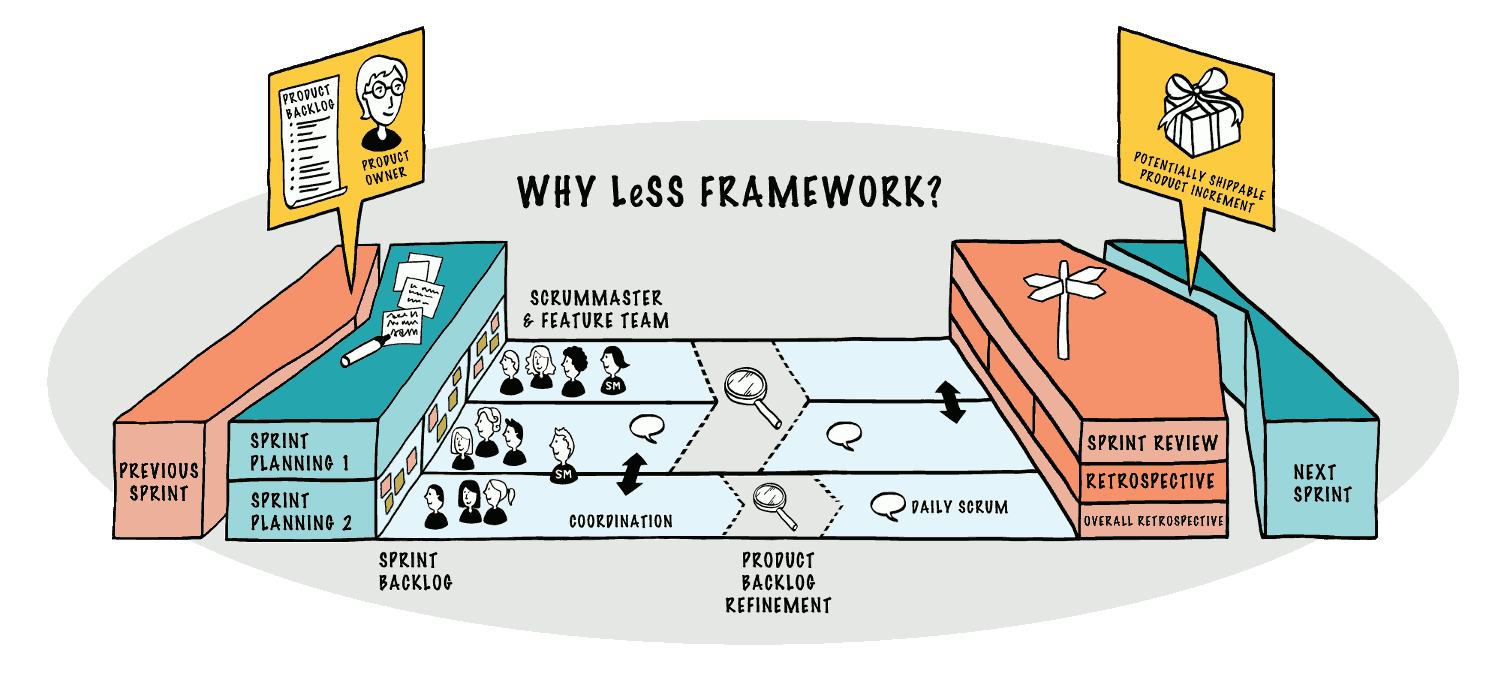
\includegraphics{Material/less_framework.png}
		%\\ Figur 1: Konceptbild på LeSS. Källa: Ramverkets webbsida. \cite{less_web}
		%\end{center}
		
	%	Några grundläggande LeSS principer är: \cite{less_principles}
	%
	%	\begin{itemize}
	%		\setlength{\itemsep}{1pt}
	%		\item LeSS är Scrum - använd Scrum-principer oförändrat i ett större sammanhang			
	%		\item Transparens
	%		\item ''\textbf{More} with \textbf{LeSS}'' dvs. \textbf{Mera} med \textbf{mindre}
	%			\begin{itemize}
	%				\item \textbf{Mer} inlärning med \textbf{mindre} definierade processer
	%				\item \textbf{Mer} värde med \textbf{mindre} omkostnader
	%				\item \textbf{Mer} ägarskap och syfte med \textbf{mindre} huvudroller och specialgrupper
	%			\end{itemize}
	%		\item Kundcentrerat
	%		\item Systemtänkande
	%	\end{itemize}
			
	\subsection{Scaled Agile Framework}
		
		Scaled Agile Framework (SAFe), skapat av Dean Leffingwell, är ett ramverk gjort för levereras av stora projekt och portföljhantering genom agil utveckling mellan flera grupper. Ramverket kan anpassas till behov, genom att lämna bort portföljaspekten till exempel.
		Centralt i SAFe är konceptet om Agile Release Trains (ART), som sammanbinder resurser, grupper och intressenter som behövs för ett specifikt mål. Inom ARTs skapas en gemensam riktning för de involverade, och gruppernas iterationer synkroniseras för gemensam leverans av produktinkrement.
		
		Byggt kring Agile Release Train strukturen
		-självorganiserade, innefattar alla nödvändiga grupper, intressenter och resurser för att kontinuerligt arbeta mot en specificerad lösning.
		-Skapar gemensam riktning för grupper, ledare och stakeholders mot ett och samma mål.
		-Levererar värdeökning i form av färdiga produktegenskaper och teknisk infrastruktur.

		Solution Train innefattar flera Agile Release Trains.
		
		Kan utökas att inkludera portföljhantering, enskilt stora projekt eller både och (Full SAFe).
				
		%todo en iteration = Program Increment, vad innefattar det
		
		%\begin{center}
		%	\includegraphics[scale=0.2]{Material/SAFeBigPicChart.jpg}
		%	\\ Figur 2: Konceptbild på SAFe. Källa: Ramverkets webbsida. \cite{safe_web}
		%\end{center}
	%	Några grundläggande SAFe principer är: \cite{safe_principles}
	%	\begin{itemize}
	%		\item Ekonomisk synpunkt
	%		\item Systemtänkande
	%		\item Förvänta förändring - bevara möjligheter
	%		\item Basera milstolpar på en objektiv värdering av ett fungerande system
	%		\item Visualisera och begränsa pågående arbete
	%	\end{itemize}
			
		
	\subsection{Disciplined Agile Delivery}
			
		Primärt skapat av Scott W. Ambler, Disciplined Agile Delivery (DAD) är ett hybrid-ramverk som utgör grunden för ett ännu bredare ramverk kallat Disciplined Agile Framework. DAD ger en samling verktyg för att skräddarsy en process för agil utveckling som passar in i de specifika omständigheterna som organisationen befinner sig i. Verktygen kommer från många andra etablerade metoder såsom Scrum, och är orsaken till att DAD kan kallas för ett hybrid-ramverk. Ramverkets specifika användningsändamål är därmed inte fastställt för att möjliggöra uppskalning, men dynamiken ger ramverket möjligheten att användas i detta syfte. Möjlighet till uppskalning listas i dokumentation som en av ramverkets största styrkor. \cite{dad_web}
		
		%todo iteration?
		
		
		
		%\begin{center}
		%	\includegraphics[scale=0.4]{Material/DAD_graphic.jpg}
		%	\\ Figur 3: DAD Konceptbild. Källa: DAD Webbsida \cite{dad_web}
		%\end{center}
			

	
	\subsection{Fallstudier}

		Fallstudier beskriver implementationer av ett ramverk i praktiken, och utgör den huvudsakliga informationen på vilken en analys kan baseras.
		Fallstudierna som behandlas i arbetet har valts på basis av deras relevans till frågeställning samt deras kvalitet. En användbar fallstudie har identifierats innehålla åtminstone resonemang kring beslutet att tillämpa agila arbetssätt i stor skala, valet av ramverk samt en beskrivning av utmaningar och resultat. Formatet på fallstudierna varierar från presentationer till intervjuer.
		Nedan följer utvalda fallstudier för de olika ramverken, kort sammanfattade.

		
		
		\subsubsection{LeSS Fallstudier}

			
			

		
		\subsubsection{SAFe Fallstudier}

			En presentation av John Plumpton från Deutsche Bank som sammanfattar bakgrunden, implementationen och resultatet av SAFe-implementationen på Deutsche Bank \cite{deutsche_case}. 
			Plumpton lyfter fram vikten av att nyckelpersonerna i implementationen är tillräckligt kvalificerade inom ramverket, i detta fall då SAFE, och betonar därmed nyttan av att ha tillgång till utomstående SAFe-konsulter. 
			Vidare understryks definitionen av roller .
			
			
			
		
		\subsubsection{DAD Fallstudier}
		
			Barclays 'Agility Capability Lead' Jonathan Smart samt produktägaren för agila antagningsgruppen Ian Dugmore intervjuas om grunderna och fördelarna av en agil transformation på Barclays\cite{barclays_interview}. Intervjun är speciellt användbar för det här arbetet då Barclays ursprungligen ställde LeSS, SAFe, och DA mot varandra och sedan valde att använda sig av DA, som i sin kärna är baserat på DAD.
			Dugmore och Smart lyfter fram flexibiliteten som DA medför, och hur viktig den är för att holistiskt kunna applicera ett ramverk i en så stor och heterogen organisation som Barclays med sina 130,000 anställda. Med holistisk menar de att agil implementation inte bara är begränsat till teknik och utveckling, utan i flera aspekter av företaget. Vidare beskriver Smart hur DA inte utesluter att på lägre nivå implementera delar av både SaFE och LeSS, men menar att dessa inte lämpar sig för att täcka hela organisationen.
			
			
		
		\subsubsection{Branscher - Data}
			
			För att kunna dra någon form av slutsats gällande vilka orsaker företag har för att välja ramverk har företagen indelats enligt bransch.
					
			Ramverk som favoriserats av en specifik bransch kan antas vara väl mer lämpat för ett dylikt företag än de andra ramverken. DAD har inte tagits i beaktande på grund av bristfällig information och total saknad av fallstudier.
			
			Observera att det inte är ändamålsenligt att jämföra statistiken sinsemellan som sådan, eftersom totala antalet fallstudier är olika. Endast de interna förhållandena mellan branscher inom ett och samma ramverk är intressanta.
				
			Nämnvärt är även att den relativt låga mängden fallstudier gör alla sorters slutsatser dragna på basis av statistiken är svaga.
			
			\title{Large Scale Scrum branscher}
			\begin{center}
				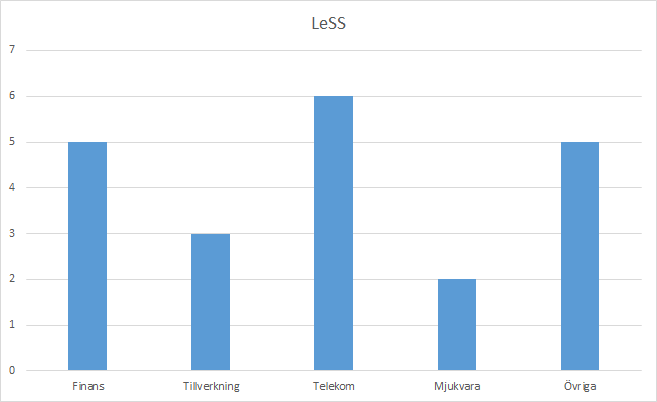
\includegraphics{Grafer/LeSS_brancher.png}
				\\ Figur 4: Brancher för fallstudier gjorda om LeSS. Källa: katalog över LeSS fallstudier \cite{less_casestudies} 
			\end{center}
		
			LeSS har en tyngdpunkt som ligger på finans och telekombranschen. Annars är det mjukvaruföretag och tillverkningsföretag som står ur mängden.\\		
				
				
			\title{Scaled Agile Framework branscher}
			\begin{center}
				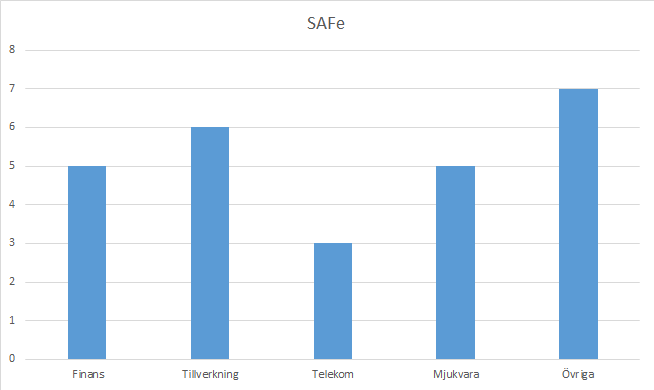
\includegraphics{Grafer/SAFe_brancher.png}
				\\ Figur 5: Brancher för fallstudier gjorde om SAFe. Källa: katalog över SAFe fallstudier \cite{safe_casestudies}
			\end{center}
					
			SAFe har lika som LeSS finansbranschen i toppen, men skiljer sig i och med att både tillverkningsföretag och mjukvaruföretag stiger över telekom.
			
		\subsubsection{Branscher - Slutsatser}
		
			Finansbranschen är återkommande för de båda stora ramverken. Inom finans finns det ovanligt höga krav på säkerhet och kvalité när det kommer till datasystem. Dels på grund av den känsliga datan men främst för att de är en vanlig målgrupp för cyber-kriminalitet. Inom finans finns det heller sällan ekonomiska hinder för projekt av tillräcklig storlek för att behöva tillämpa ett ramverk för uppskalning. 
			
			Institutioner för finans, såsom banker, kan således konstateras vara bland de första som haft både behov och resurser att implementera ramverken.
			
			
			Skillnad i popularitet mellan telekom- och tillverkningsbranschen kan tänkas bero på skilda behov i respektive bransch. Telekom arbetar med en mångfald olika system, medan tillverkning ofta har utmaningar relaterade till logistik och tydliga processer, såsom löpande band.
			
	

	\subsection{Popularitet och adoption}
	
		Mängden tillgängligt material ger en riktgivande uppfattning om i vilken utsträckning ramverken används. Mer entydig data finns dock för att stöda uppfattningen och för att ge en tydligare bild.
		
		Enligt en rapport baserad på en enkät gjort av Version one är SAFe betydligt mer utbrett jämfört med LeSS och DAD. \cite{version_one_report} \\	
		
		Observera att man i själva enkäten kunde kryssa flera alternativ, därav en totalprocent på mer än hundra:
		
		\begin{center}
			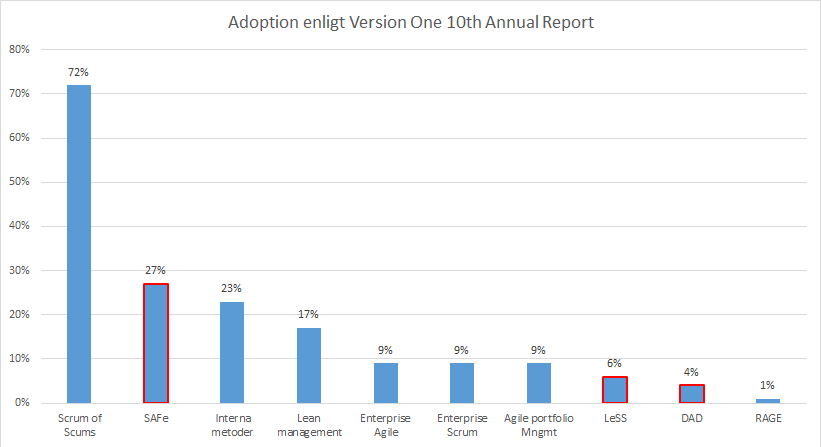
\includegraphics{Grafer/AnnualReport_Adoption.png}
			\\Figur 6: Statistik för adoptionen av metoder för uppskalning av agil utveckling. Källa: Version one rapport. \cite{version_one_report}
		\end{center}
		
	
		Den egenskap som korrelerar starkast med ett ramverks eller metods popularitet i ovanstående rapport är kostnad. De mest populära ramverken och metoderna i Version One rapporten har även en implementationskostnad listad som 'låg' i Agile Scaling Knowlegde -matrisen. \cite{ask_matrix}				
		Såsom det påpekas i kapitlet om Material och Metoder går många av de populära metoderna inte att klassificera som ramverk. 
		
		
		Resultatet från enkäten öppnar inte direkt huruvida ramverken är populära jämfört med varandra, förutom att SAfE är i en klass för sig. Sökmotorn Google ger statistik på popularitet av olika över tiden. I egenskap av världens mest populära sökmotor ger denna statistik en god uppfattning om huruvida ett ramverk är allmänt känt och använt eller ej. 
		
		Då alla tre ramverks sökningar sätts emot varandra kan det igen konstateras att det SAFe är klart mer eftersökt. Ur samma data syns DAD och LeSS som lika eftersökta.
		
		Y-axeln är ett automatiskt genererat jämförelsetal direkt korrelerande med antal sökningar per tidsenhet. Resultaten ger således endast interna förhållanden, och är inte absoluta.
		\begin{center}
			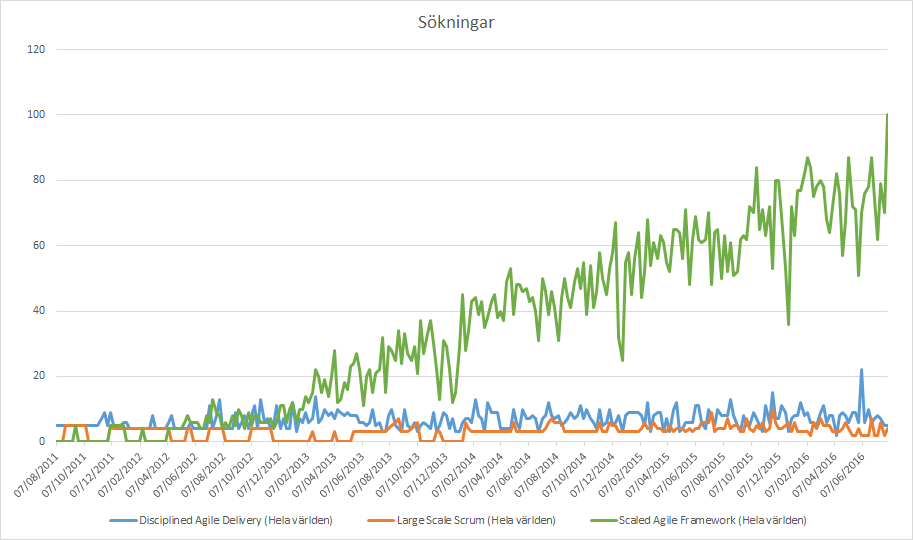
\includegraphics{Grafer/Google_sokningar.png}
			\\ Figur 7: Graf över google sökningar. Källa: Google Stats \cite{google_stats}
		\end{center}
	
	
		Genom att utesluta SAFe får man ett noggrannare resultat för LeSS och DAD, vilket är mer ändamålsenligt. DAD genomgår en positivare trend, och är i allmänhet mera eftersökt än LeSS. Detta är motstridigt mot det resultat som rapporterades i Version One rapporten. Detta kan tyda på ett mer utvidgat intresse för DAD i framtiden, då trenden för dess popularitet är klart positiv jämfört med LeSS.
	
		Y-axeln är igen ett jämförelsetal som endast är menat för intern jämförelse inom denna graf.
		\begin{center}
			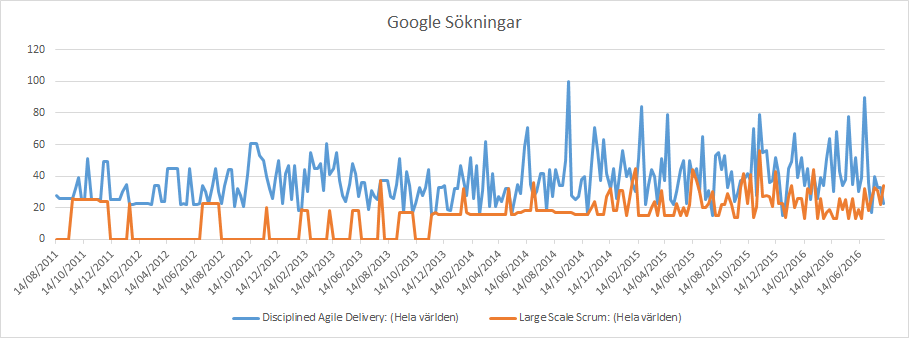
\includegraphics{Grafer/Google_sokningar_dad_less.png}
			\\ Figur 8: Graf över google sökningar. Källa: Google Stats \cite{google_stats_dad_less}
		\end{center}
		
		
	
\section{Analys}

	\subsection{Jämförelse}
		
		DAD kan tänkas kräva mera kunskap, då beslutet om verktygen som ska användas slutligen faller på användaren.
		
		Föreskrivande (prescriptive) ställt mot mål-drivna val. Flexibilitet på bekostnad av användarvänlighet.
		
		Barclay valde DAD tack vare dess flexibiltet (inte ett "one size fits all" ramverk)
		==> En komplicerad företagsstruktur krävde en skräddarsydd lösning. 
		\cite{barclays_interview}
		
		
		
		Skillnader i iteration (DAD iterations-centrerat, vad föreskriver det?)
	
	\subsection{Användningsområden}
	
	
	
	\subsection{Diskussion och fortsatt forskning}
		Att göra en betydelsefull jämförelse av så omfattande ramverk som detta arbete presenterar är utmanande. Tillgänglig information finns främst i form av hela böcker samt webbsidor, och bygger på mycket bakgrundskunskap. En relevant analys vore bäst baserad på praktisk erfarenhet av ramverken.
		I detta arbete kunde ingen djup analys göras, på grund av arbetes storlek och avsaknaden av forskning i området.
		
		
		Dock kan man på ytan se skillnader i bland annat popularitet och användningsområden. SAFe ligger starkt först i popularitet, både ur företagens och agil-konsulters synvinkel.
		Konsulterna verkar visa mer intresse för DAD, trots att LeSS används mera bland företag. Detta tyder på att DAD möjligtvis kommer åt att användas mer brett i framtiden.
		
		
		Märkbart är även att ramverken i stort sett har samma principer enligt vilka de fungera, dock med skilda prioriteter och praktiska arrangemang.
		
		
		Finns mycket kvar att göra i fråga om forskning i ramverk för agil utveckling. Främst kunde analyser och konkreta sammanfattningar av de enskilda ramverken göras, som sedan kunde möjliggöra mer djupgående och betydelsefull jämförelse. Dock kan konstateras att med endast ramverkens rådata till hands och inga studier, är en jämförelse ett arbetsamt och utmanande projekt.
		
	

	